\chapter{Stakeholder Analysis} \label{ch:Stakeholder Analysis}

This project focuses on being a small R\&D team at Grundfos. In this team the installation and management of the newly implemented robot is of high value.\\
The team wants to ensure the interest and power for the future stakeholders of this project.\\
It is important to know where the information for the project is located. This is why stakeholder-Analysis is important.\\
When it is known who the stakeholders are and what they require of interest/power, it will be easier to locate the data that is needed for a good assignment.\\

%The purpose of the stakeholder analysis, is to give an overview of which groups could have an interest and power to influence the design of a new robotic cell.\\
%\\

The stakeholders can be split into 4 different groups, depending on their amount of interest, and power to influence.\\
The groups are: Key-Players, Keep Informed, Suppliers and Keep Satisfied.\\
\section{Different players}

\subsection{Key-Players}
The purpose of the key players, are that they have to be managed closely, thus also requiring regular meetings and updates about the progress of the design process.\\

\subsection{Keep Informed}
The purpose of this group is, that they usually have low power to influence the project, but has a great interest in it, and its impact.\\

\subsection{Suppliers}
This group usually has low power and interest in the project, as the biggest impact it can have on them is if the project is a success, they might get bigger orders for materials in the future.\\

\subsection{Keep Satisfied}
This group can have a high impact on the project, because they are sitting in places that have power to influence the direction of the project, but it is not of their primary concern, so they are designated by having high power, but low interest.\\

\begin{figure}[h]
    \centering
    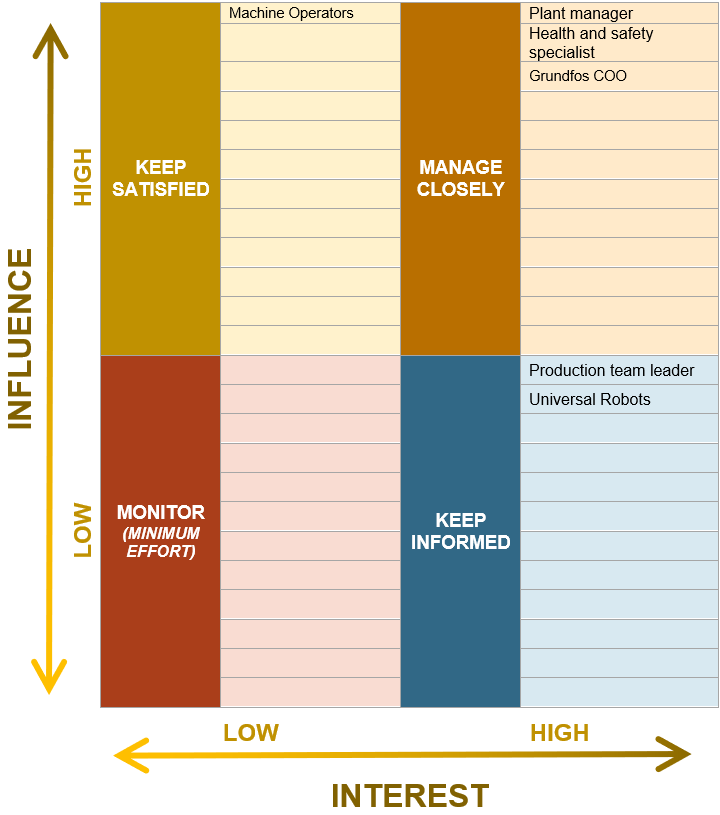
\includegraphics[width=9cm]{StakeholderAnalysis/SWOT.PNG}
    \caption{SWOT analysis}
    \label{fig:SWOT analysis}
\end{figure}


\section{Stakeholders}


\subsection{Grundfos COO}\label{ch:grundfosas-CEO}
Stéphane Simonetta is the Chief Operating Officer of Grundfos. The COO is responsible for the supply-chain, manufacturing and purchase.\\ 
He create operations and policies, while communicating with the employees about the corporate goals.\\
The COO has a high power and high interest. When planning a new work-cell in the company, it has to collaborate with the whole production-line. Therefore the COO has the power to set it in motion or deny it.\cite{Grundfos},\cite{COO}\\

\subsection{Plant manager}\label{ch:Plant-manager} 
The plant manager has the responsibility of all the robots, and is in charge of keeping them running smoothly. It is his job to replace old robots, and making sure they are all up to date. Therefore, a new work-cell would also be in interest. It is the plant managers job to hire new personnel, assign workers and training them, so he would also be interested in the simplicity of the robots, and that would make the training of new personnel much easier. \cite{plantmanager} \\

\subsection{Production team leader}\label{ch:Production-team-leader}
The production team leader is responsible for the safety and training of all personnel in the production area, as well as making sure the output complies to the requirements, and is of sufficient quality. The production team leader is also responsible for ensuring maintenance and order in the production line. For these reasons, the production team leader has a high interest, but low power in terms of influencing the development of the product. \cite{Productionteamleader}


\subsection{Operator}\label{ch:grundfosemp-stake}
An operator is a person who is responsible of the automated robots running properly in his area and restarting the robots if they should make an error. This person has a high influence and low power, they need to be kept satisfied \cite{Operator}.\\

\subsection{Health and Safety Specialists}\label{ch:SafetyPersonel}

H&S Specialists is required when installing new machinery. They have a say in everything that is put on Grundfos' floor globally.\\
Senior manager, Marie Kloppenborg Jensen, says that she experiences Grundfos' high prioritization towards H&S. Hereby the H&S managers should be key-players since the work-cell has to be managed closely by the safety specialists \cite{H&S}.\\

\subsection{Universal Robots}\label{ch:Universalrobots-stake}
The suppliers of the robotic manipulator in this case has a high interest and a low power.\\The reason is if we should choose their manipulator over a competitors manipulator, they can then adjust the prices on the manipulator so we would choose their product in this case. \\


\section{Conclusion}
As a small R\&D group the stakeholders has been managed as seen above. To get a good and collaborative process, the group will need the conscent of the key-players, and keep the others in the loop as well. 
%\subsection{The Public}\label{ch:Public-stake}
%The public has low interest and low power, their interest mostly concerns, reading up on new designs and technology being made.

%\subsection{Aalborg University}\label{ch:Aau-stake}
%Aalborg University has an interest in the development of robotics from a research and information perspective. For this reason they potentially have an interest in investing in further development and improvement of a technology such as the UR. 